%%%%%%%%%%%%%%%%%% GENERATED DISSERTATION SOURCE %%%%%%%%%%%%%%%%%%
% Generated from the optimized Markdown copy in final draft.
% Original template files were copied before modification.

\begin{filecontents*}{\jobname.xmpdata}
  \Title{A Two-Layer Decision-Making System for Vehicle Lane Changing Based on Reinforcement Learning}
  \Author{14226506}
  \Language{en-GB}
  \Copyrighted{True}
\end{filecontents*}

\documentclass[11pt,msc]{uom_eee_dissertation_casson}

\usepackage{graphicx}
  \graphicspath{ {./images/} }
\usepackage{amsmath}
  \allowdisplaybreaks[1]
\usepackage{amssymb}
\usepackage{url}
\usepackage{float}
\usepackage{booktabs}
\usepackage{longtable}
\usepackage{array}
\usepackage{tabularx}
\usepackage{multirow}
\usepackage{subcaption}
\usepackage{siunitx}
\usepackage[base]{babel}

\newcommand{\degree}{\ensuremath{^\circ}}
\newcommand{\sus}[1]{$^{\mbox{\scriptsize #1}}$}
\newcommand{\sub}[1]{$_{\mbox{\scriptsize #1}}$}
\newcommand{\otoprule}{\midrule[\heavyrulewidth]}
\newcolumntype{Z}{>{\centering\arraybackslash}X}

\usepackage[style=ieee,backend=biber,backref=true,hyperref=auto,maxbibnames=3,minbibnames=1]{biblatex}
\DefineBibliographyStrings{english}{backrefpage = {cited on p\adddot}, backrefpages = {cited on pp\adddot}}
\addbibresource{references.bib}

\quickwordcount{\currfilebase}

\begin{document}
\makeatletter
\title{\xmp@Title}
\studentid{\xmp@Author}
\makeatother

\course{Robotics}
\faculty{Science and Engineering}
\school{School of Engineering}
\submitdate{2026}
\wordcount{\mywordcount}
\maketitle

\uomtoc

\begin{abstract}
Lane changing is a fundamental problem in autonomous driving. This dissertation proposes a two-layer decision-making and control framework for autonomous vehicles to merge into the target lane. The proposed method decomposes the lane changing problem into two coupled but functionally distinct layers: the upper-level module determines which local gap is preferable, while the lower-level module converts the selected gap into continuous target points and actual vehicle control inputs. The upper-level module uses only the three target-lane vehicles closest to the ego vehicle, forms two candidate gaps with these three vehicles, evaluates the relative feasibility of the two gaps through a smooth confidence function, and updates the upper-level opinion state using the opinion dynamics equation with reinforcement terms. The lower-level module further calculates the objective bias based on the size and rate of change of the selected gap, uses a SAC policy to determine the attention intensity, updates the lower-level opinion state, and maps this opinion to the target control points within the gap. Finally, the front-axle tracking controller generates vehicle acceleration and angular velocity changes.

Simulation experiments are implemented in Python to evaluate the proposed control method. The experimental results show that in a single-gap environment, the reinforcement learning method of SAC learns an effective strategy and maintains convergence, and the vehicle can successfully complete the task; in a multi-gap environment, the policy learned in the simple environment transfers to the more complex setting, and the effectiveness of the two-layer decision-making system is verified.
\end{abstract}
\clearpage

\begin{uomoriginality}
  \uomoriginalitydeclaration
\end{uomoriginality}
\uomcopyrightstatement

\begin{uomacknowledgements}
Acknowledgements may be added here.
\end{uomacknowledgements}

\uomstartmainbody

\chapter{Introduction}



\section{Background and Motivation}



\subsection{Decision-making strategies for merge and lane-change interaction}





Lane-changing decisions are representative problems in autonomous driving. A lane change alters the available gaps, road right-of-way expectations, and future responses of surrounding vehicles. Recent research has therefore increasingly treated lane changing as an interactive perception decision task. Game theory models are widely used because they can explicitly describe the strategic relationship between the ego vehicle and surrounding vehicles. Lane changing intentions, collision probabilities, and dynamic risks can be incorporated into the payoff function to determine whether a maneuver is beneficial or dangerous \cite{R1,R2}. Physics-inspired models such as molecular interaction potentials further express the attraction and repulsion between vehicles as continuous interaction forces \cite{R3}. Recent studies also consider incomplete information and social driving preferences, as in lane changing conflicts involving human-driven vehicles, surrounding vehicles may exhibit cooperative, aggressive, or uncertain behaviors \cite{R4}.



Another important direction is learning-based interactive prediction. Graph neural networks and attention mechanisms represent vehicles as nodes and the influence between vehicles as edges or attention weights. This is highly suitable for lane changing scenarios, as the number and importance of surrounding vehicles will dynamically change. Existing research uses topological graphs combined with driving behavior and traffic context to predict the lane changing intentions of drivers \cite{R5}, and some studies use plan-aware graph attention networks to predict the responses of surrounding vehicles to the candidate intentions of the ego vehicle, and then the model predicts the control trajectory \cite{R6}. These methods illustrate that interaction modeling should not only predict where other vehicles will go, but also estimate how they will respond to the ego vehicle's decision. Cooperative control methods provide a third route. In connected autonomous driving environments, surrounding vehicles can actively create gaps, coordinate lane changing sequences, or maintain fleet stability \cite{R7,R8}. Overall, recent literature provides motivation for the hierarchical framework: this framework requires the combination of strategy interaction modeling, behavior prediction, and safe execution.



\subsection{Reinforcement learning for adaptive decision dynamics}





The lane-changing decision-making process exhibits sequentiality, uncertainty, and feedback-driven characteristics. Vehicles need to determine when to wait, when to change lanes, and how to adjust their speed. Traditional fixed-parameter controllers may perform well in static scenarios, but they often lack flexibility when the traffic environment changes or when the system needs to switch between cooperative consensus and competitive divergence. Deep reinforcement learning provides a mechanism for learning decision strategies through repeated interactions. Existing studies have integrated safety rules, future risk assessment, reward shaping, and robust observation modeling into DRL lane-changing strategies \cite{R9,R10,R11}. These studies show that RL should not be used as an unconstrained black box, but should be guided by interpretable state variables, safety-aware reward terms, and robust mechanisms.



Meanwhile, MARL allows each connected or autonomous vehicle to learn from the behavior of neighboring vehicles while considering system-level outcomes such as traffic efficiency, comfort, and safety \cite{R12}. Right-of-way coordination and Mix Q-learning further illustrate that the lane-changing task can balance individual benefits with group benefits \cite{R13,R14}. For this dissertation, these studies support a key idea: RL is not just a direct output of lane-changing actions, but can dynamically adjust the control parameters of the nonlinear decision dynamics model. This enables adaptive changes according to environmental stimuli while still maintaining connection with low-level safety control.



\subsection{Evaluation dimensions: from efficiency to safety, comfort, and adaptability}





The evaluation of lane-changing decisions has shifted from a single efficiency metric to a multi-dimensional assessment. Average speed, travel time, traffic volume, and lane-changing success rate remain important, but they are not sufficient to support safety-critical autonomous driving systems. A rapid lane change can still be unsafe, uncomfortable, or disrupt the traffic flow. Therefore, recent research has begun to evaluate collision risk, minimum distance, braking feasibility, safety violation rate, acceleration, deceleration, traffic flow stability, and robustness under perception uncertainty \cite{R7,R8,R10,R15}. This project adopts these evaluation perspectives, which emphasize convergence speed, safety violation rate, and task efficiency while also evaluating safety, comfort, and stability.





\section{Aims and Objectives}





The aim of this project is to develop, integrate, and evaluate a hierarchical decision-making and control framework for interactive autonomous driving scenarios. This framework will use reinforcement learning to adjust the key parameters of the nonlinear decision dynamics/control model, enabling the agent to quickly make decisions in the simulation environment while meeting safety constraints.



This project has five specific objectives. First, it establishes a nonlinear opinion dynamics model at the policy layer. Second, it trains the agent using RL methods to dynamically optimize the model parameters. Third, it develops a safety perception and execution layer, using control barrier functions or equivalent constraints to convert the high-level policy into collision-free trajectories. Fourth, it implements the controller in the Python simulation framework. Fifth, it compares with the baseline and evaluate the decision-control effectiveness.



\chapter{Methods}





The controller adopts a two-layer structure. The upper-layer controller completes the discrete control problem of gap selection through the evaluation of different gaps and the update of opinion dynamics; the lower-layer controller, solves the continuous control problem of actual vehicles using the actual size and change rate of the gap, as well as the attention parameters learned by reinforcement learning.



\begin{figure}[H]
\centering

\includegraphics[width=0.92\linewidth]{System_block_diagram.png}
\caption{Control system structure block diagram}
\label{fig:system-block-diagram}
\end{figure}



Fig. 1: Control system structure block diagram



\section{High-Level Control System}

\subsection{Opinion Dynamics and Self-Updating Attention}





The same opinion-dynamics template \cite{R16} is used at both levels. As shown in the following formula, for the general opinion variable \(o(t)\), its dynamics are defined below, where the damping coefficient \(d > 0\) pulls the opinion back to the neutral position to prevent it from drifting infinitely; the attention intensity \(u(t) \geq 0\) determines the degree to which the existing opinion is self-reinforced; the sensitivity parameter \(\alpha > 0\) determines the speed at which the nonlinear term enters the saturation zone; the external bias \(b(t)\) injects the environmental evaluation into the system. If \(b(t)\) is close to zero, the damping term will cause the opinion to decay; if there is a small but persistent bias, the self-reinforcement term will gradually amplify the opinion until a stable decision is formed.



\[

\dot{o}(t) =

-d\,o(t)

+u(t)\tanh\!\left(\alpha o(t)\right)

+b(t).

\[





The dynamics of the high-level decision opinion can be expressed in the following form, where \(y(t)\) represents the opinion of the high-level decision-making.



\[

\dot{y}(t) =

-d_y y(t)

+u_h(t)\tanh\!\left(\alpha_y y(t)\right)

+B(t).

\[





In high-level decision-making, the external environment bias is determined by the gap confidence, while attention is updated by the following self-updating law. This Hill-type function depends on \(y^2\), so the sign of the opinion is treated symmetrically. When \(y(t)\) approaches zero, attention decays and the vehicle remains cautious; when \(|y(t)|\) increases, \(S_h\) rises, thereby increasing \(u_h(t)\), and a larger \(u_h(t)\) further strengthens the self-reinforcing term in the opinion equation. This feedback loop enables small but continuous preferences to gradually transform into stable gap selection.



\[

\dot{u}_h(t) =

\frac{-u_h(t)+S_h(y(t)^2)}{\tau_h},

\[



\[

S_h(y^2) =

U_{\max}

\frac{(y^2)^n}{K_h^n+(y^2)^n}.

\[



\subsection{High-Level Bias from Gap Confidence}





At each time step, the high-level module selects the three target-lane vehicles closest to the ego front axle in the longitudinal coordinate. Let these vehicles be ordered from front to rear as \((i_1,i_2,i_3)\). The forward candidate gap is the space between \(i_1\) and \(i_2\), and the rear candidate gap is the space between \(i_2\) and \(i_3\). For any candidate gap formed by a front vehicle \(F\) and a rear vehicle \(R\), the gap center and gap velocity are



\[

x_g(t) =

\frac{p_F^x(t)+p_R^x(t)}{2},

\[



\[

v_g(t) =

\frac{v_F^x(t)+v_R^x(t)}{2}.

\[





The ego-to-gap alignment is defined by the longitudinal position error and the relative speed error:



\[

d_g(t) =

x_g(t)-p_e^x(t),

\[



\[

\Delta v_g(t) =

v_g(t)-v_e^x(t).

\[





The confidence of a gap is then evaluated using a Gaussian radial-basis function:



\[

C_g(t) =

\exp

\left(

-\frac{d_g(t)^2}{2\sigma_d^2}

-\frac{\Delta v_g(t)^2}{2\sigma_v^2}

\right).

\[





When the gap center is close to the ego vehicle and the relative speed is low, the confidence level is higher; when the gap is spatially far apart or the speed matching is poor, the confidence level smoothly decreases. The forward and rear confidences are converted into a signed directional bias:



\[

B(t) =

C_f(t)-C_r(t).

\[





The difference is used because they retain both the direction and intensity of the preference. If \(B(t) > 0\), it indicates that the front gap is more consistent with the current ego state; if \(B(t) < 0\), it indicates that the rear gap is more in line; if \(B(t) \approx 0\), it means the evidence is still ambiguous. Even if the absolute values of the two confidence levels are both small, the difference between them can still represent a weak but meaningful relative preference. Through the opinion dynamics equation, this weak preference will only accumulate and gradually become clearer when it persists. This keeps the comparison process smooth and makes the decision changes more stable.



\subsection{High-Level Opinion Update and Decision Mapping}





The high-level opinion \(y(t)\) stores the accumulated directional belief. After computing \(B(t)\) and updating \(u_h(t)\), the system integrates the high-level opinion using an explicit time step \(\Delta t\), and updates the attention:



\[

y_{k+1} =

y_k

+\Delta t

\left[

-d_y y_k

+u_{h,k}\tanh(\alpha_y y_k)

+B_k

\right].

\[



\[

u_{h,k+1} =

u_{h,k}

+\Delta t

\frac{-u_{h,k}+S_h(y_k^2)}{\tau_h}.

\[





The high-level decision mapping is threshold-based, and the decision is made according to the following rule:



\[

\mathrm{decision}_k =

\begin{cases}

\mathrm{forward}, & y_k>\theta_y,\\

\mathrm{rear}, & y_k<-\theta_y,\\

\mathrm{wait}, & |y_k|\leq\theta_y.

\end{cases}

\[





The waiting interval prevents frequent changes in the selected gap when \(C_f\) and \(C_r\) are close, allowing vehicles to leave the neutral zone and make a choice only after sufficient evidence has accumulated. Therefore, this mechanism is smoother than the direct instantaneous comparison. Even if the group selection of the vehicle closest to the ego vehicle changes, the decision will not suddenly change due to a jump in confidence, which is more consistent with the actual driving behavior logic.



\begin{figure}[H]
\centering

\includegraphics[width=0.92\linewidth]{layered_opinion_decision_schematic.png}
\caption{layered\_opinion\_decision\_schematic}
\label{fig:layered-opinion-decision-schematic}
\end{figure}



Fig. 2: Layered opinion decision schematic



\section{Low-Level Control System}





After the high-level module selects a candidate gap, the low-level module decides how the ego vehicle should enter that gap. The low-level module first evaluates the physical feasibility of the selected gap, then determines the attention intensity, updates the low-level opinion \(z(t)\), and finally converts \(z(t)\) into continuous target points. This design makes the merging action gradual: as the low-level opinion strengthens, the target points gradually move from the original lane reference position to within the selected gap.



\subsection{Low-Level Bias}





For a selected gap formed by a front vehicle \(F\) and a rear vehicle \(R\), the physical gap length and  gap-rate term is



\[

g(t) =

p_F^x(t)-p_R^x(t).

\[



\[

\dot{g}(t) =

v_F^x(t)-v_R^x(t).

\[





The low-level bias evaluates whether the gap is sufficiently large and whether it is opening or closing:



\[

b(t) =

k_g\left[g(t)-g_{\mathrm{safe}}\right]

+k_v\dot{g}(t).

\[





A larger gap makes \(b(t)\) more positive. An opening gap, where \(\dot{g}(t)>0\), also increases \(b(t)\). A small or closing gap decreases \(b(t)\), delaying the growth of the low-level merge intention. This formula is intentionally interpretable: \(g(t)-g_{\mathrm{safe}}\) measures spatial feasibility, while \(\dot{g}(t)\) measures whether the situation is improving or worsening.



\begin{longtable}{p{0.22\linewidth}p{0.22\linewidth}p{0.22\linewidth}}
\toprule
Gap condition & Mathematical effect & Control meaning \\
\midrule
Large and opening & \(g>g_{\mathrm{safe}},\ \dot{g}>0\) & Positive bias, stronger merge tendency \\
Large but closing & \(g>g_{\mathrm{safe}},\ \dot{g}<0\) & Moderate bias, cautious merge tendency \\
Small and opening & \(g<g_{\mathrm{safe}},\ \dot{g}>0\) & Waiting may be appropriate \\
Small and closing & \(g<g_{\mathrm{safe}},\ \dot{g}<0\) & Negative bias, merge should be suppressed \\
\bottomrule
\end{longtable}



\subsection{The attention obtained through reinforcement learning}





The low-level attention \(u(t)\) regulates the intensity of the self-reinforcement of the low-level opinions. However, the optimal timing of attention is difficult to design manually because the system simultaneously contains nonlinear opinion dynamics, moving vehicles, safety avoidance, input saturation, and delay consequences. If attention is increased too early, the ego vehicle may overcommit when the gap is not yet safe; if attention is increased too late, the vehicle may miss the merging opportunity and behave too conservatively. Therefore, reinforcement learning is used to learn the temporal sequence of attention from the reward feedback. At the same time, the learned strategy does not replace the model controller, but only outputs the attention variables in the opinion dynamics. This action space is low-dimensional and interpretable.



\subsection{SAC Reinforcement Learning Design}





Soft Actor-Critic is an off-policy actor-critic algorithm suitable for continuous action spaces. It learns the random policy \(\pi_\phi(a|s)\), two soft Q functions, and the entropy temperature parameter. Its optimization objective is to balance between the expected return and the policy entropy:

The entropy term promotes exploration, which is crucial for the lane-changing task because a useful policy not only needs to learn to stay safe but also needs to learn when to actively make a lane change.



\[

J(\pi) =

\sum_{t}

\mathbb{E}_{(s_t,a_t)\sim\rho_{\pi}}

\left[

r(s_t,a_t)

+\alpha_{\mathrm{SAC}}\mathcal{H}\left(\pi(\cdot|s_t)\right)

\right].

\[





The low-level reinforcement-learning state describes the relative geometry and velocity between the ego vehicle and the front and rear vehicles of the selected gap. The state is defined as follows. Here \(F\) and \(R\) denote the front and rear vehicles of the selected gap.



\[

s_t =

\begin{bmatrix}

\Delta x_F &

\Delta y_F &

\Delta v_F^x &

\Delta v_F^y &

\Delta x_R &

\Delta y_R &

\Delta v_R^x &

\Delta v_R^y

\end{bmatrix}^{\top}.

\[





The policy output is the low-level attention:



\[

a_t =

u(t),

\qquad

u(t)\in[u_{\min},u_{\max}].

\[





The reward function is designed to encourage timely merging, discourage hesitation, penalize oscillatory motion, and strongly penalize collision. A representative per-step reward is



\[

\begin{aligned}

r_t

=&

w_p\,\Delta P_t

+w_o\,O_t\max(\Delta P_t,0)

-w_h\,O_t(1-P_t)

-w_s(1-P_t) \\

&

-w_a\lVert a_t-a_{t-1}\rVert_2^2

-w_f\,\mathbb{I}\!\left[v_y(t)v_y(t-1)<0\right] \\

&

-w_c

\left[

\max\left(0,\frac{d_{\mathrm{safe}}-d_{\min}(t)}{d_{\mathrm{safe}}}\right)

\right]^2

-1000\,\mathbb{I}_{\mathrm{collision}}

+R_{\mathrm{success}}(t)\,\mathbb{I}_{\mathrm{success}} .

\end{aligned}

\[





Lane-changing progress is defined as the normalized ratio:



\[

P_t =

\mathrm{clip}

\left(

\frac{y_e(t)-y_O}{y_T-y_O},

0,

1

\right),

\qquad

\Delta P_t=P_t-P_{t-1}.

\[





The opportunity term \(O_t\) represents whether the selected gap is currently suitable for merging. The progress terms reward moving toward the target lane, especially when a useful opportunity exists. The hesitation terms penalize remaining far from the target lane, so the policy cannot receive a high score by simply waiting. The action-smoothness and direction-flip terms reduce repeated acceleration or lateral-direction reversals. The safety term is continuous before collision, while the collision term is a large terminal penalty. The success bonus decreases with time, for example



\[

R_{\mathrm{success}}(t) =

100-2t,

\[





\begin{longtable}{p{0.22\linewidth}p{0.22\linewidth}}
\toprule
Reward term & Meaning \\
\midrule
\(w_p\Delta P_t\) & Rewards direct lane-change progress \\
\(w_oO_t\max(\Delta P_t,0)\) & Gives extra reward for moving during a valid opportunity \\
\(-w_hO_t(1-P_t)\) & Penalizes hesitation when a gap is available \\
\(-w_s(1-P_t)\) & Applies a general time / inaction penalty \\
\(-w_a\lVert a_t-a_{t-1}\rVert_2^2\) & Penalizes abrupt action changes \\
\(-w_f\mathbb{I}[v_y(t)v_y(t-1)<0]\) & Penalizes lateral direction flips \\
Safety distance penalty & Penalizes near-collision continuously \\
Collision penalty & Strong terminal penalty \\
Success bonus & Rewards early safe completion \\
\bottomrule
\end{longtable}



\subsection{Low-Level Opinion and Target Point}





The low-level opinion \(z(t)\) represents the degree of merge commitment for the selected gap. Its continuous dynamics and discrete update are



\[

\dot{z}(t) =

-d_z z(t)

+u(t)\tanh\!\left(\alpha_z z(t)\right)

+b(t).

\[



\[

z_{k+1} =

z_k

+\Delta t

\left[

-d_z z_k

+u_k\tanh(\alpha_z z_k)

+b_k

\right].

\[





A low or negative \(z(t)\) keeps the desired target point close to the original lane or a cautious reference. A high positive \(z(t)\) moves the target point toward the selected gap in the target lane. To keep this transition bounded, \(z(t)\) is mapped through a smooth gate:



\[

\lambda_z(t) =

\mathrm{clip}

\left(

\frac{z(t)-z_{\min}}{z_{\max}-z_{\min}},

0,

1

\right).

\[



\section{Actual Control Input}





The final control layer converts the desired target point into actual vehicle input. This layer consists of three parts: a safety obstacle avoidance item that pushes the ego vehicle away from the nearby target lane vehicles, a tracking error pointing to the desired target point, and a reverse solution of the bicycle model that maps the desired front axle acceleration to longitudinal acceleration and angular rate of change. Through explicit safety constraints and vehicle kinematics expressions, the entire system becomes safer and more interpretable.



\subsection{Safety-Avoidance Term}





For each surrounding target-lane vehicle \(j\), define the relative vector from that vehicle to the ego front axle as



\[

\mathbf{r}_j(t) =

\mathbf{p}_e(t)-\mathbf{p}_j(t),

\qquad

d_j(t) =

\lVert \mathbf{r}_j(t)\rVert_2.

\[





The safety-avoidance acceleration is constructed as a repulsive field:



\[

\mathbf{u}_c(t) =

\sum_j

k_c

\max\left(0,\frac{d_{\mathrm{safe}}-d_j(t)}{d_{\mathrm{safe}}}\right)^2

\frac{\mathbf{r}_j(t)}{d_j(t)}.

\[





When all vehicles are farther than \(d_{\mathrm{safe}}\), this term is zero. When a vehicle enters the safety region, the repulsive magnitude grows quadratically as distance decreases. This term does not replace collision checking; instead, it provides a continuous pre-collision correction that can steer the ego vehicle away before a hard collision boundary is reached.



\subsection{Target Point and Tracking Error}





The selected-gap target point is usually placed near the longitudinal center of the gap and at the target-lane center. The original-lane reference point can be placed ahead of the ego vehicle along the original lane:



\[

\mathbf{p}_G^{\star}(t) =

\begin{bmatrix}

x_g(t) \\

y_T

\end{bmatrix}.

\[



\[

\mathbf{p}_O^{\star}(t) =

\begin{bmatrix}

p_e^x(t)+\ell_{\mathrm{look}} \\

y_O

\end{bmatrix}.

\[





The opinion-weighted target point and tracking error are:



\[

\mathbf{p}^{\star}(t) =

\left[1-\lambda_z(t)\right]\mathbf{p}_O^{\star}(t)

+\lambda_z(t)\mathbf{p}_G^{\star}(t).

\[



\[

\mathbf{e}_z(t) =

\mathbf{p}^{\star}(t)-\mathbf{p}_e(t).

\[





This construction gives the low-level opinion a direct geometric meaning. When \(\lambda_z(t)\) is close to zero, the controller behaves like a lane-keeping controller. When \(\lambda_z(t)\) approaches one, the controller behaves like a gap-entry controller.



\subsection{Final Physical Input Design}





The desired front-axle acceleration combines proportional position tracking, velocity damping, and safety avoidance:



\[

\mathbf{u}_{\mathrm{total}}(t) =

k_p\mathbf{e}_z(t)

-k_v\mathbf{v}_e^f(t)

+\mathbf{u}_c(t).

\[





This vector is then converted into physical inputs. Let the front-axle velocity direction and its normal direction be



\[

\mathbf{t}_e(t) =

\frac{\mathbf{v}_e^f(t)}

{\lVert\mathbf{v}_e^f(t)\rVert_2+\epsilon},

\qquad

\mathbf{n}_e(t) =

\begin{bmatrix}

-t_e^y(t) \\

t_e^x(t)

\end{bmatrix}.

\[





The longitudinal acceleration can be approximated by projection onto \(\mathbf{t}_e\):



\[

a(t) =

\mathrm{clip}

\left(

\mathbf{u}_{\mathrm{total}}(t)^{\top}\mathbf{t}_e(t),

a_{\min},

a_{\max}

\right).

\[





The steering-rate command is generated from the lateral component:



\[

\omega(t) =

\mathrm{clip}

\left(

k_{\omega}\,

\mathbf{u}_{\mathrm{total}}(t)^{\top}\mathbf{n}_e(t),

\omega_{\min},

\omega_{\max}

\right).

\[





This PID-like structure provides a clear and stable mapping from the opinion-driven target point to the executable vehicle input, while avoiding unrealistic acceleration and steering changes through input clipping.



\chapter{Experimental Design}





The experiments are organized from simple to complex. The single gap environment isolated the low-level control problem: testing the learning effect of RL when the target gap is fixed, and whether the controller can learn when to increase attention and commit to merging. The multi-gap environment introduced high-level decisions: when multiple dynamic gaps exist simultaneously, whether the system can select the appropriate local gap to avoid excessive switching and safely execute merging. The experimental parameters are listed in the appendix.



\section{Single-Gap Merging Experiment}





The single-gap environment contains one front vehicle, one rear vehicle, and one ego vehicle. The front and rear vehicles travel in the target lane, and their longitudinal separation defines the only available merging gap. The ego vehicle starts from the original lane and attempts to merge into this gap. The lane width is \(W=4.0\,\mathrm{m}\), so the original and target lane centers are \(y_O=0.5W=2.0\,\mathrm{m}\) and \(y_T=1.5W=6.0\,\mathrm{m}\), respectively. The initial target-vehicle states are



\[

x_F(0)=30.0\,\mathrm{m},\qquad

x_R(0)=15.0\,\mathrm{m},\qquad

v_F(0)=v_R(0)=15.0\,\mathrm{m/s}.

\[





The ego vehicle has the same initial longitudinal speed but a randomized longitudinal initial position. This randomization makes the training and evaluation less dependent on one special initial alignment. It forces the policy to learn an attention schedule that works when the ego vehicle starts slightly ahead of or behind the gap center.



\[

x_e(0)=20.0+\xi,\qquad

\xi\sim\mathcal{U}(-5.0,5.0),\qquad

y_e(0)=2.0\,\mathrm{m},\qquad

v_e(0)=15.0\,\mathrm{m/s}.

\[





The rear vehicle is deliberately designed to create a staged merging opportunity. Before \(t_y=20.0\,\mathrm{s}\), the rear vehicle follows a sinusoidal acceleration law. Let



\[

\omega_s=\frac{2\pi}{P_s},\qquad

P_s=6.0\,\mathrm{s},\qquad

A_s=4.0\,\mathrm{m/s}.

\[





For \(0\leq t\leq t_y\), the rear-vehicle acceleration, velocity, and position are



\[

a_R(t)=A_s\omega_s\cos(\omega_s t),

\[



\[

v_R(t)=v_R(0)+A_s\sin(\omega_s t),

\[



\[

x_R(t)=x_R(0)+v_R(0)t+\frac{A_s}{\omega_s}\left[1-\cos(\omega_s t)\right].

\[





Since the front vehicle travels with constant speed \(v_F=15.0\,\mathrm{m/s}\), the front-rear gap before yielding is therefore



\[

g(t)=x_F(t)-x_R(t)

=15.0-\frac{A_s}{\omega_s}\left[1-\cos(\omega_s t)\right],

\qquad

0\leq t\leq20.0.

\[





After \(20.0\,\mathrm{s}\), the rear vehicle starts yielding by tracking a desired front-rear gap \(g_{\mathrm{yield}}=20.0\,\mathrm{m}\). The rear-vehicle acceleration becomes:



\[

a_R(t)=

\mathrm{clip}

\left(

0.35\left[g(t)-20.0\right]

-1.1\left[v_R(t)-v_F(t)\right],

-5.0,

2.0

\right),

\qquad

t>20.0.

\[





Equivalently, the gap dynamics after yielding are governed by



\[

\dot{g}(t)=v_F(t)-v_R(t),

\qquad

\ddot{g}(t)=-a_R(t),

\qquad

t>20.0.

\[





This piecewise construction has a clear purpose. Before \(20.0\,\mathrm{s}\), the gap is not intentionally opened for the ego vehicle, so the policy should avoid premature aggressive merging. After \(20.0\,\mathrm{s}\), the rear vehicle creates a larger gap and the correct behavior is to increase attention \(u(t)\), allow the opinion \(z(t)\) to grow, and move the target point toward the target lane.





The SAC agent uses a Gaussian policy with two hidden layers of width \(256\), two Q networks, target Q networks, replay-buffer learning, and entropy regularization. The main training parameters are \(200\) episodes, replay-buffer size \(2.0\times10^5\), batch size \(256\), \(1000\) initial random steps, discount factor \(\gamma=0.99\), target-update rate \(\tau=0.005\), and learning rates \(3\times10^{-4}\) for the policy, Q networks, and entropy temperature. The subsequent value comparison is also carried out using the same "reward" as defined in the previous text. The same reward definition is used during value comparison so that the learned and hand-designed policies are judged by an identical metric. The baseline comparison evaluates the trained SAC attention against the original hand-designed RBF attention:



\[

u_{\mathrm{RBF}}(t)=

u_{\mathrm{base}}+

u_{\mathrm{amp}}

\exp

\left(

-\frac{d_g(t)^2}{2\sigma_d^2}

-\frac{\Delta v_g(t)^2}{2\sigma_v^2}

\right).

\[





The evaluation repeats the simulation \(100\) times with shared random ego initial positions. For each random seed, both policies face the same initial \(x_e(0)\) and the same target-vehicle trajectory. The comparison reports the episode reward of each trial and the mean and standard deviation across trials:



\[

\bar{R}_{\mathrm{SAC}}=\frac{1}{N_{\mathrm{eval}}}\sum_{j=1}^{N_{\mathrm{eval}}}R_{\mathrm{SAC}}^{(j)},

\qquad

\bar{R}_{\mathrm{RBF}}=\frac{1}{N_{\mathrm{eval}}}\sum_{j=1}^{N_{\mathrm{eval}}}R_{\mathrm{RBF}}^{(j)},

\qquad

N_{\mathrm{eval}}=100.

\[



\section{Multi-Gap Merging Experiment}



\begin{figure}[H]
\centering
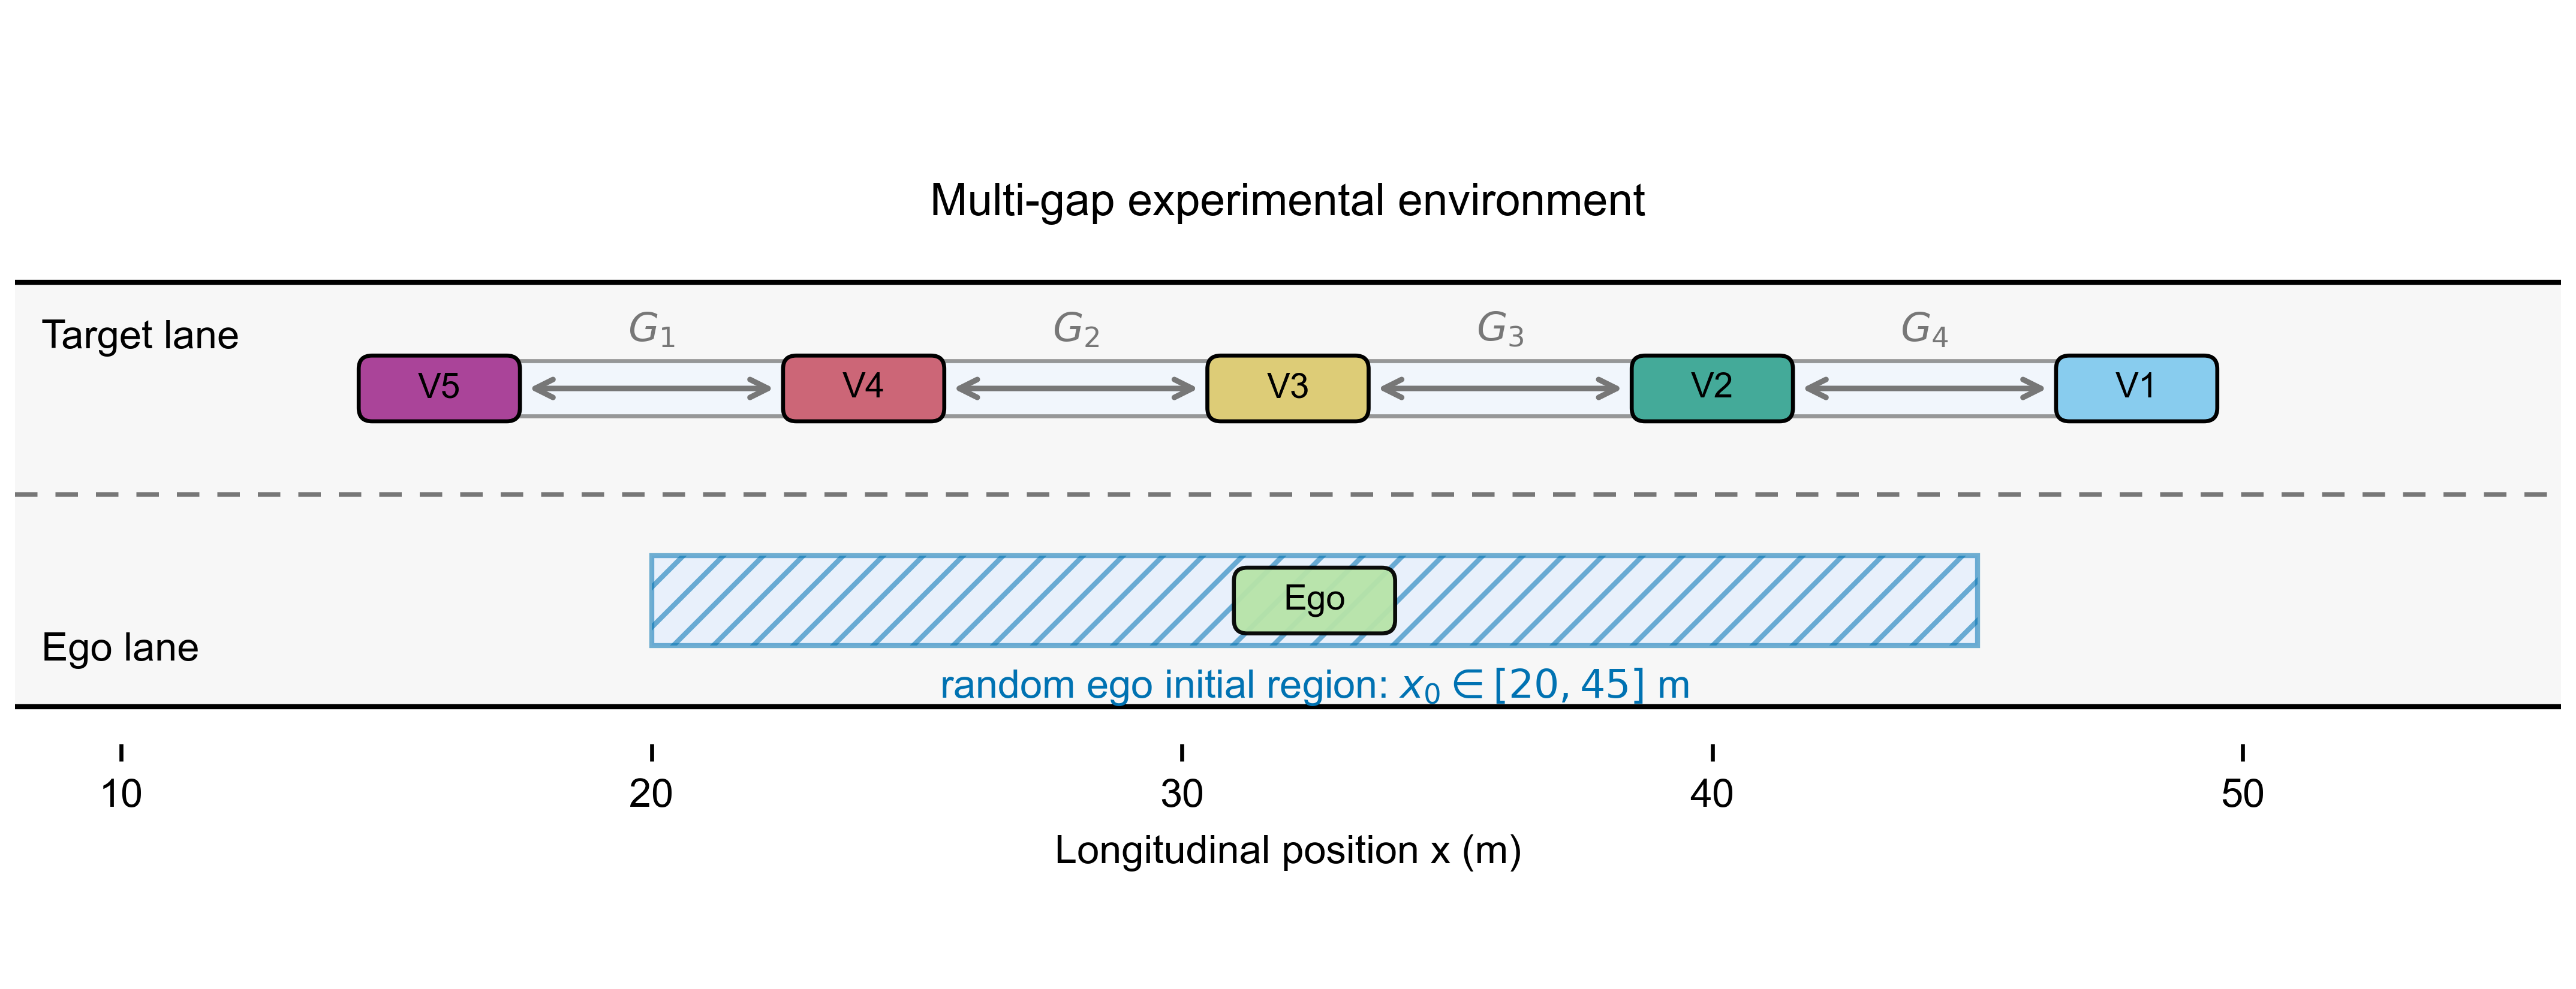
\includegraphics[width=0.92\linewidth]{multi_gap_environment_schematic.png}
\caption{multi\_gap\_environment\_schematic}
\label{fig:multi-gap-environment-schematic}
\end{figure}



Fig. 3: Multi gap environment schematic





The multi-gap environment extends the same merging task to a target lane containing five vehicles and four physical gaps. The target vehicles are initialized with a uniform base spacing:



\[

N=5,\qquad

x_i(0)=48.0-(i-1)g_0,\qquad

g_0=8.0\,\mathrm{m},\qquad

i=1,\ldots,5.

\[





All target vehicles start on the target-lane center \(y_T=6.0\,\mathrm{m}\) with nominal speed \(15.0\,\mathrm{m/s}\). The ego vehicle starts from the original lane with a larger longitudinal randomization range than in the single-gap experiment. The larger random range changes which three vehicles are nearest to the ego vehicle at the beginning of an episode. Therefore, the high-level selector must work under different local traffic configurations rather than repeatedly facing one fixed gap.





\[

x_e(0)=30.0+\xi,\qquad

\xi\sim\mathcal{U}(-10.0,15.0),\qquad

y_e(0)=2.0\,\mathrm{m},\qquad

v_e(0)=15.0\,\mathrm{m/s}.

\[





The four target-lane gaps are randomly adjusted over time. Every \(T_g=4.0\,\mathrm{s}\), at most two gaps are selected for modification, and each selected gap receives a desired spacing from the multiplier set



\[

\mathcal{M}=\{0.75,1.0,1.25,1.5\}.

\[





The leading target vehicle has zero acceleration. Each following target vehicle tracks the desired gap in front of it through a clipped proportional-derivative rule:



\[

a_{i+1}(t)=

\mathrm{clip}

\left(

0.55\left[g_i(t)-g_{i,\mathrm{des}}^{(k)}\right]

 +1.05\dot{g}_i(t),

-4.0,

4.0

\right).

\[





This mechanism produces a target lane in which gaps open, close, and reconfigure during the \(40.0\,\mathrm{s}\) simulation. The high-level decision module selects the nearest three target-lane vehicles in longitudinal front-axle coordinate and compares the two local gaps formed by these vehicles. The multi-gap experiment is designed to evaluate generalization. The underlying strategy uses the attention strategy learned in the single-gap environment. This design tests whether a strategy that only learns \(u(t)\) for a single pair of preceding and following vehicles remains effective when the high-level selector continuously provides different pairs of preceding and following vehicles. If the strategy is generalizable, then even if the gap selection and gap environment change, the ego vehicle should still be able to smoothly enter the selected gap.





The high-level ablation compares the opinion-dynamics selector with a simple maximum-score selector. The maximum-score baseline removes the high-level opinion memory and chooses the locally better gap instantaneously:



\[

i_k^{\star}=\arg\max_i S_i(t_k),

\[





where \(S_i(t_k)\) is the instantaneous confidence or gap-evaluation score of candidate gap \(i\). The proposed opinion-dynamics selector instead integrates the confidence difference over time:



\[

\dot{y}(t)=-d_y y(t)+u_h(t)\tanh(\alpha_y y(t))+C_f(t)-C_r(t).

\[





This comparison was evaluated through multiple random ablation experiments. The current test setup uses \(N_{\mathrm{test}} = 100\) random runs. For each method, the total reward and the number of times the selected gap was switched were compared.



\chapter{Results and discussion}



\section{Single-gap SAC Training}



\begin{figure}[H]
\centering
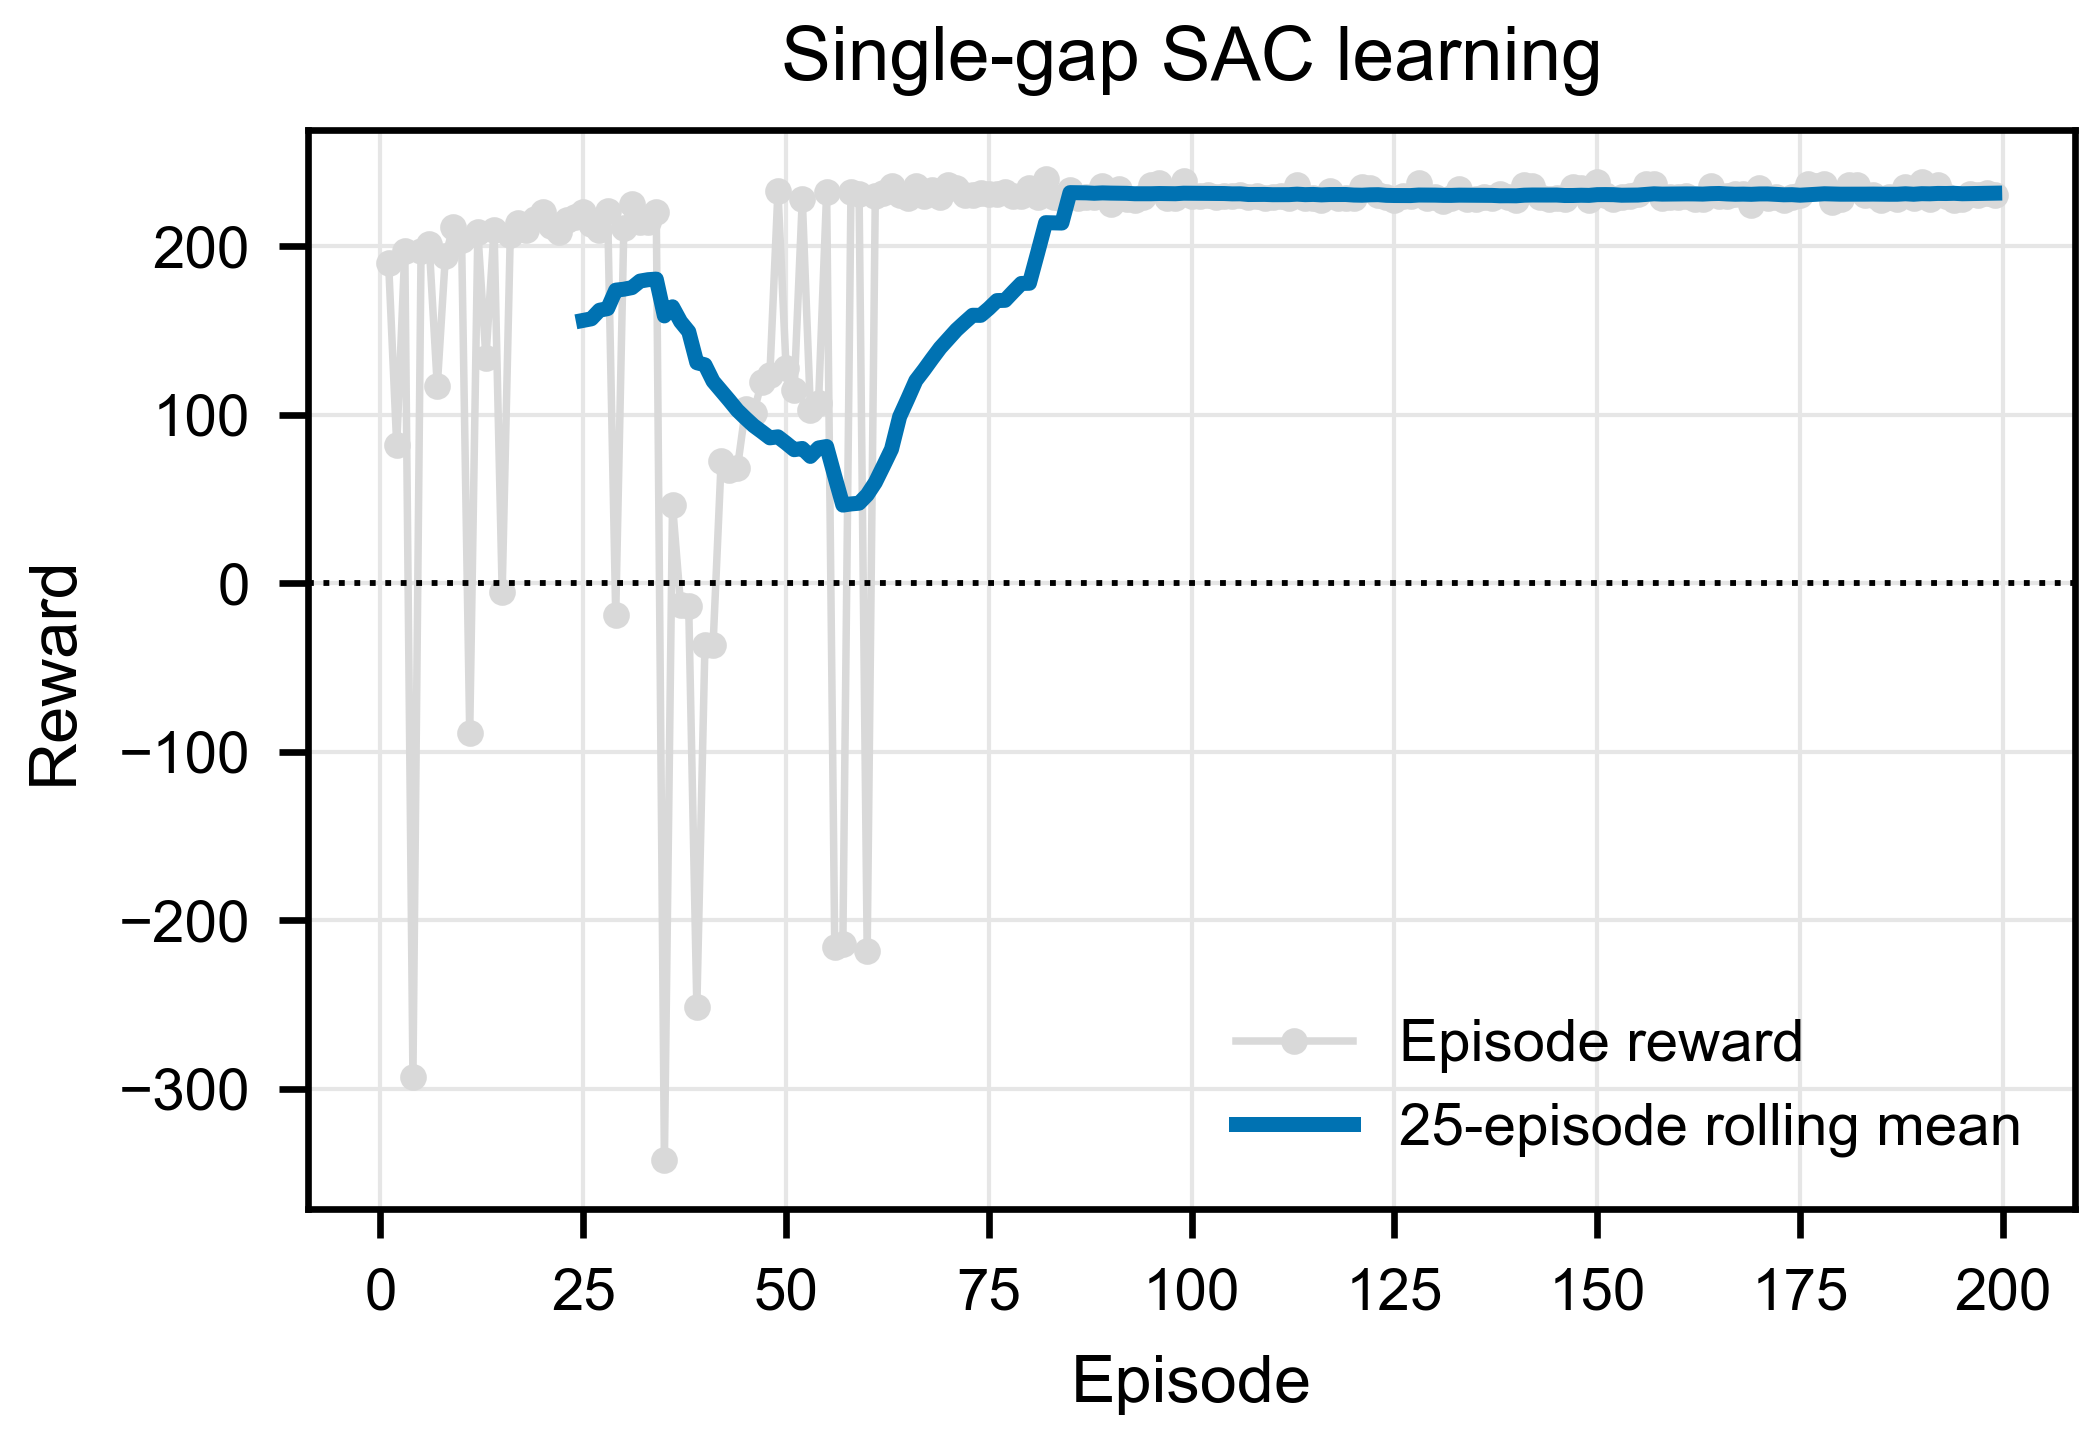
\includegraphics[width=0.92\linewidth]{fig1_single_gap_training.png}
\caption{fig1\_single\_gap\_training}
\label{fig:fig1-single-gap-training}
\end{figure}



Fig. 4: Single-gap training reward





The training results show that in the initial 50 episodes, the algorithm conducted extensive exploration, resulting in significant fluctuations in the reward. The algorithm converged after 50 episodes. The SAC agent converged within 50 episodes, achieving a stable episodic reward of 230\(\pm\)10 (Fig. 4). The Q1-loss decreased from an initial peak of 134 to below 20, indicating accurate value function    approximation. The entropy coefficient \(\alpha\) decayed monotonically from 0.96 to 0.12, confirming a smooth transition from exploration to exploitation. The policy consistently reached the target gap (progress \(\geq\) 0.95) with a 97.5\% success rate (195/200) and zero collisions. The average control command (mean\_u) stabilized around 1.9, suggesting an efficient, non-conservative driving policy. These results demonstrate that SAC effectively learns a robust and safe gap-acceptance strategy.



\section{Comparison with Baseline RBF Controller}



\begin{figure}[H]
\centering
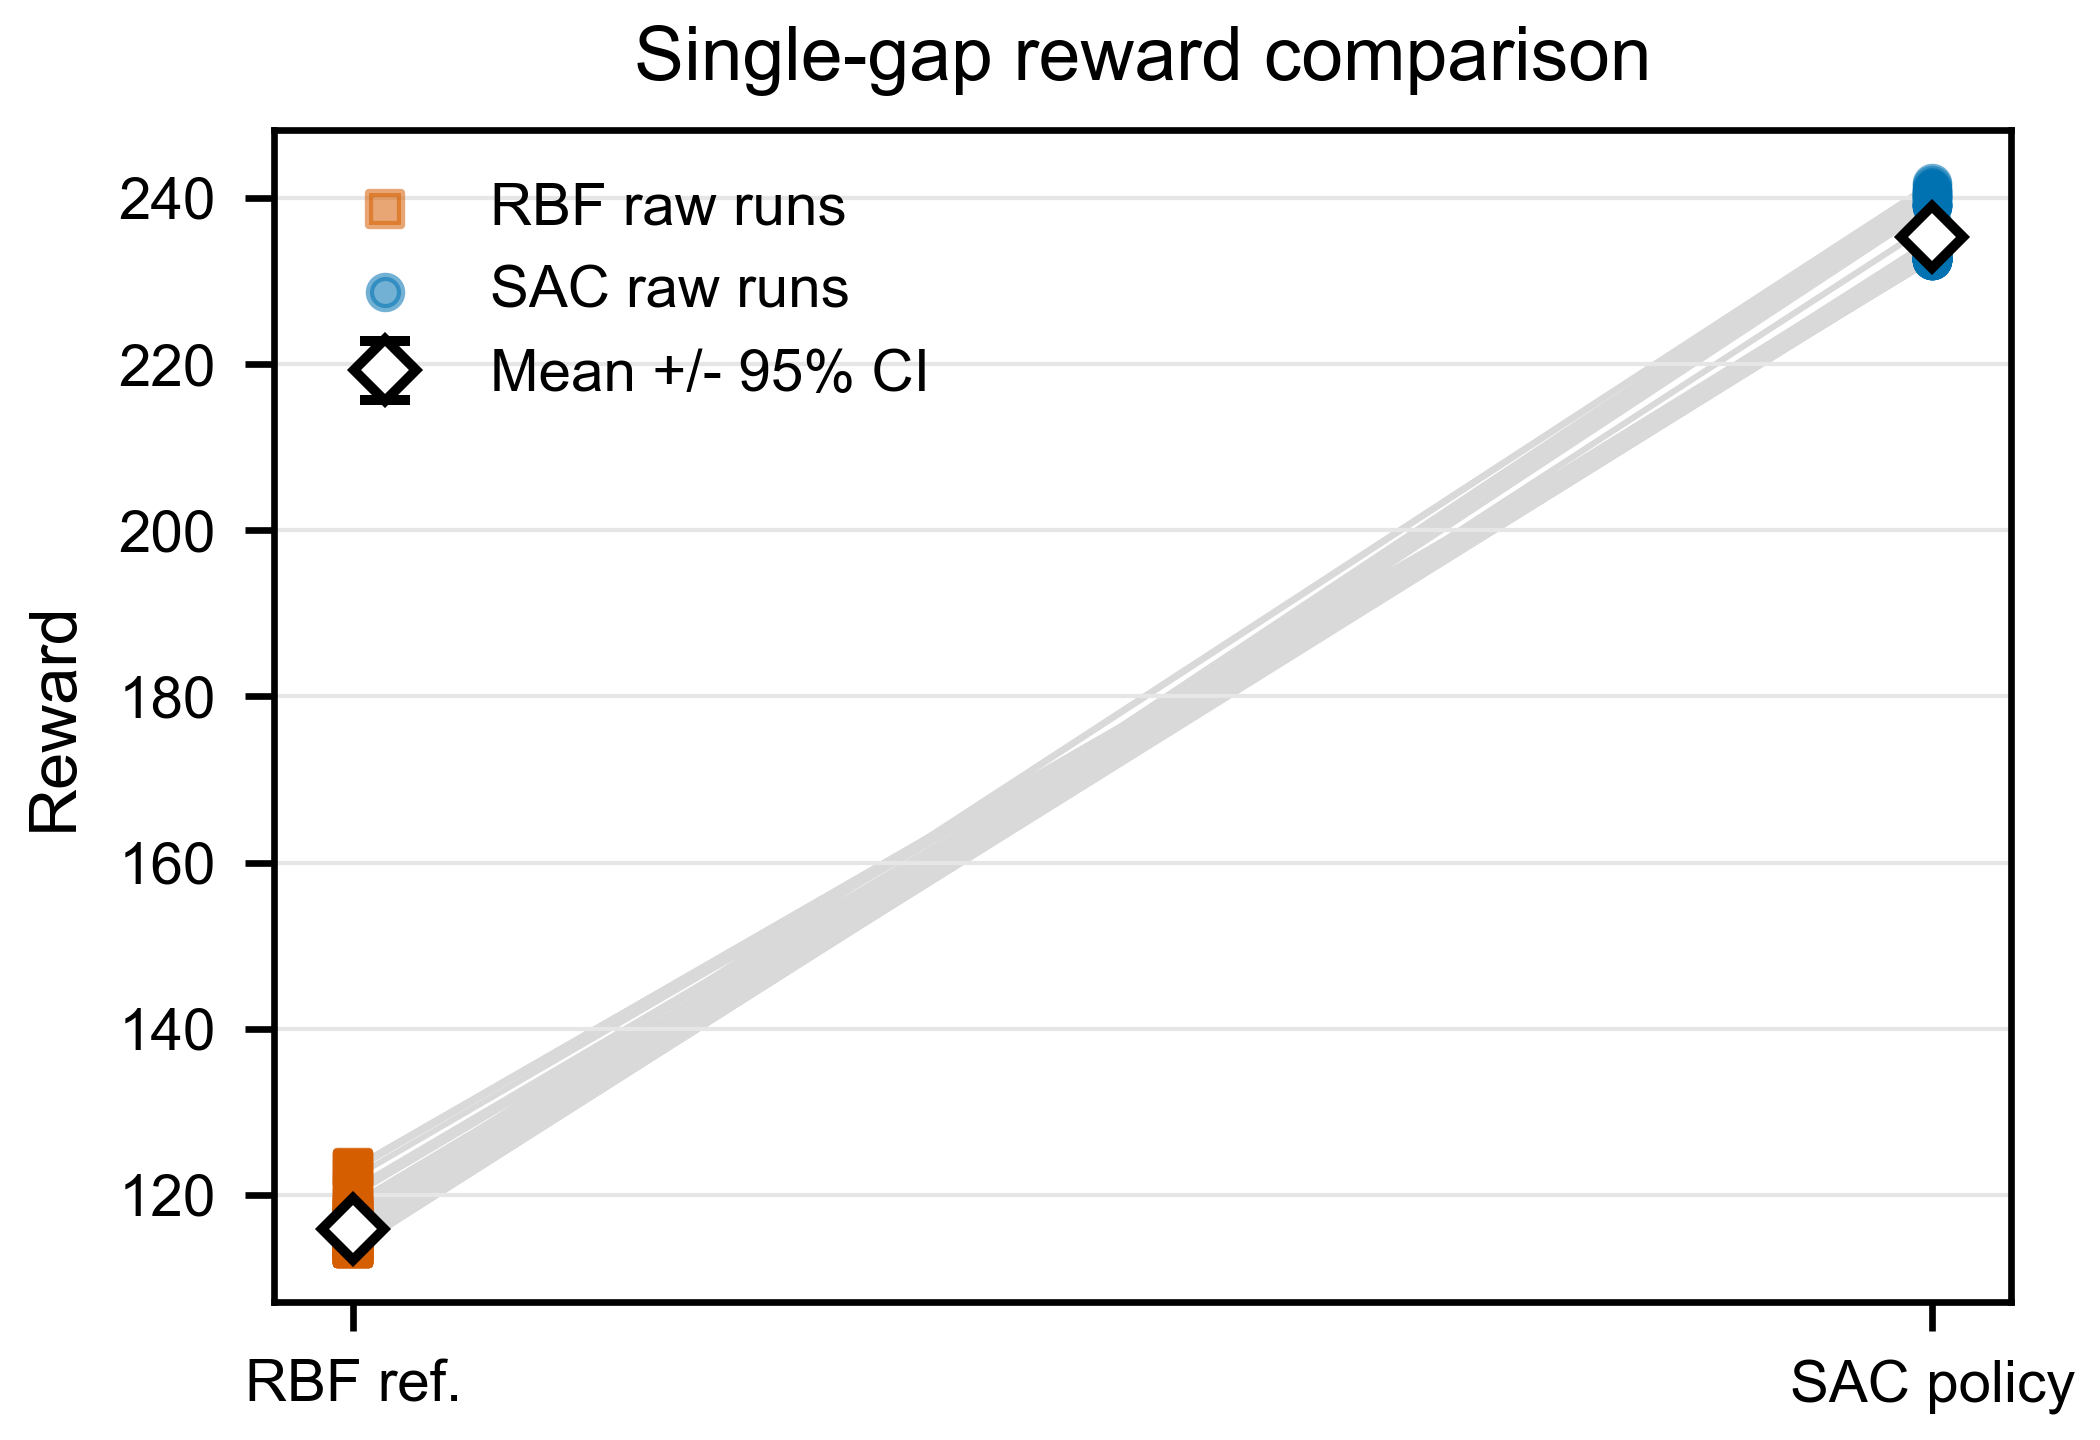
\includegraphics[width=0.92\linewidth]{fig2_single_gap_policy_vs_rbf.png}
\caption{fig2\_single\_gap\_policy\_vs\_rbf}
\label{fig:fig2-single-gap-policy-vs-rbf}
\end{figure}



Fig. 5: Comparison between SAC and RBF reward





Compared with the manually designed baseline, the quantitative results are shown in the table. The SAC strategy achieved significantly higher average episodic reward ($\textbackslash{}bar\{R\}\_\{\textbackslash{}mathrm\{SAC\}\} = 233.4$), while the RBF baseline was only ($\textbackslash{}bar\{R\}\_\{\textbackslash{}mathrm\{RBF\}\} = 115.8$), with an average increase of approximately 117.6 points. Although both strategies achieved 100\% success rate and no collisions, the most significant difference lies in the efficiency of task execution. The SAC strategy only takes an average of 6.9 seconds to select the lane change gap. In contrast, the RBF controller consumes 29.45 seconds per round of testing, which is very close to the preset simulation time limit. This indicates that although the RBF manual rules ensure safety, the strategy is overly conservative and fails to fully utilize the longitudinal motion capability of the vehicle. While SAC agent has learned an aggressive but safe strategy, reducing the task completion time by over 75\%.



In terms of safety indicators, the RBF baseline maintained a larger minimum distance ($d\_\{\textbackslash{}min\} \textbackslash{}approx 9.7$ m), reflecting its inherent conservatism. The SAC strategy is closer to the obstacle ($d\_\{\textbackslash{}min\} \textbackslash{}approx 2.6$ m), but always remains outside the collision radius, proving that the learned strategy can effectively balance time efficiency and collision safety through an optimized reward structure.



\begin{longtable}{p{0.22\linewidth}p{0.22\linewidth}p{0.22\linewidth}p{0.22\linewidth}}
\toprule
Metric & SAC Policy & RBF Baseline & Improvement \\
\midrule
\textbf{Episodic Reward} ($\textbackslash{}bar\{R\}$) & \textbf{$233.4 \textbackslash{}pm 4.2$} & $115.8 \textbackslash{}pm 2.1$ & \textbf{+101.5\%} \\
\textbf{Task Time (s)} & \textbf{$6.9 \textbackslash{}pm 0.2$} & $29.45 \textbackslash{}pm 2.4$ & \textbf{-76.6\%} \\
\textbf{Success Rate} & 100\% & 100\% & — \\
\textbf{Collision Rate} & 0\% & 0\% & — \\
\textbf{Min. Distance (m)} & $2.62 \textbackslash{}pm 0.23$ & $9.70 \textbackslash{}pm 0.01$ & — \\
\bottomrule
\end{longtable}



\section{Multi-Gap}



\begin{figure}[H]
\centering
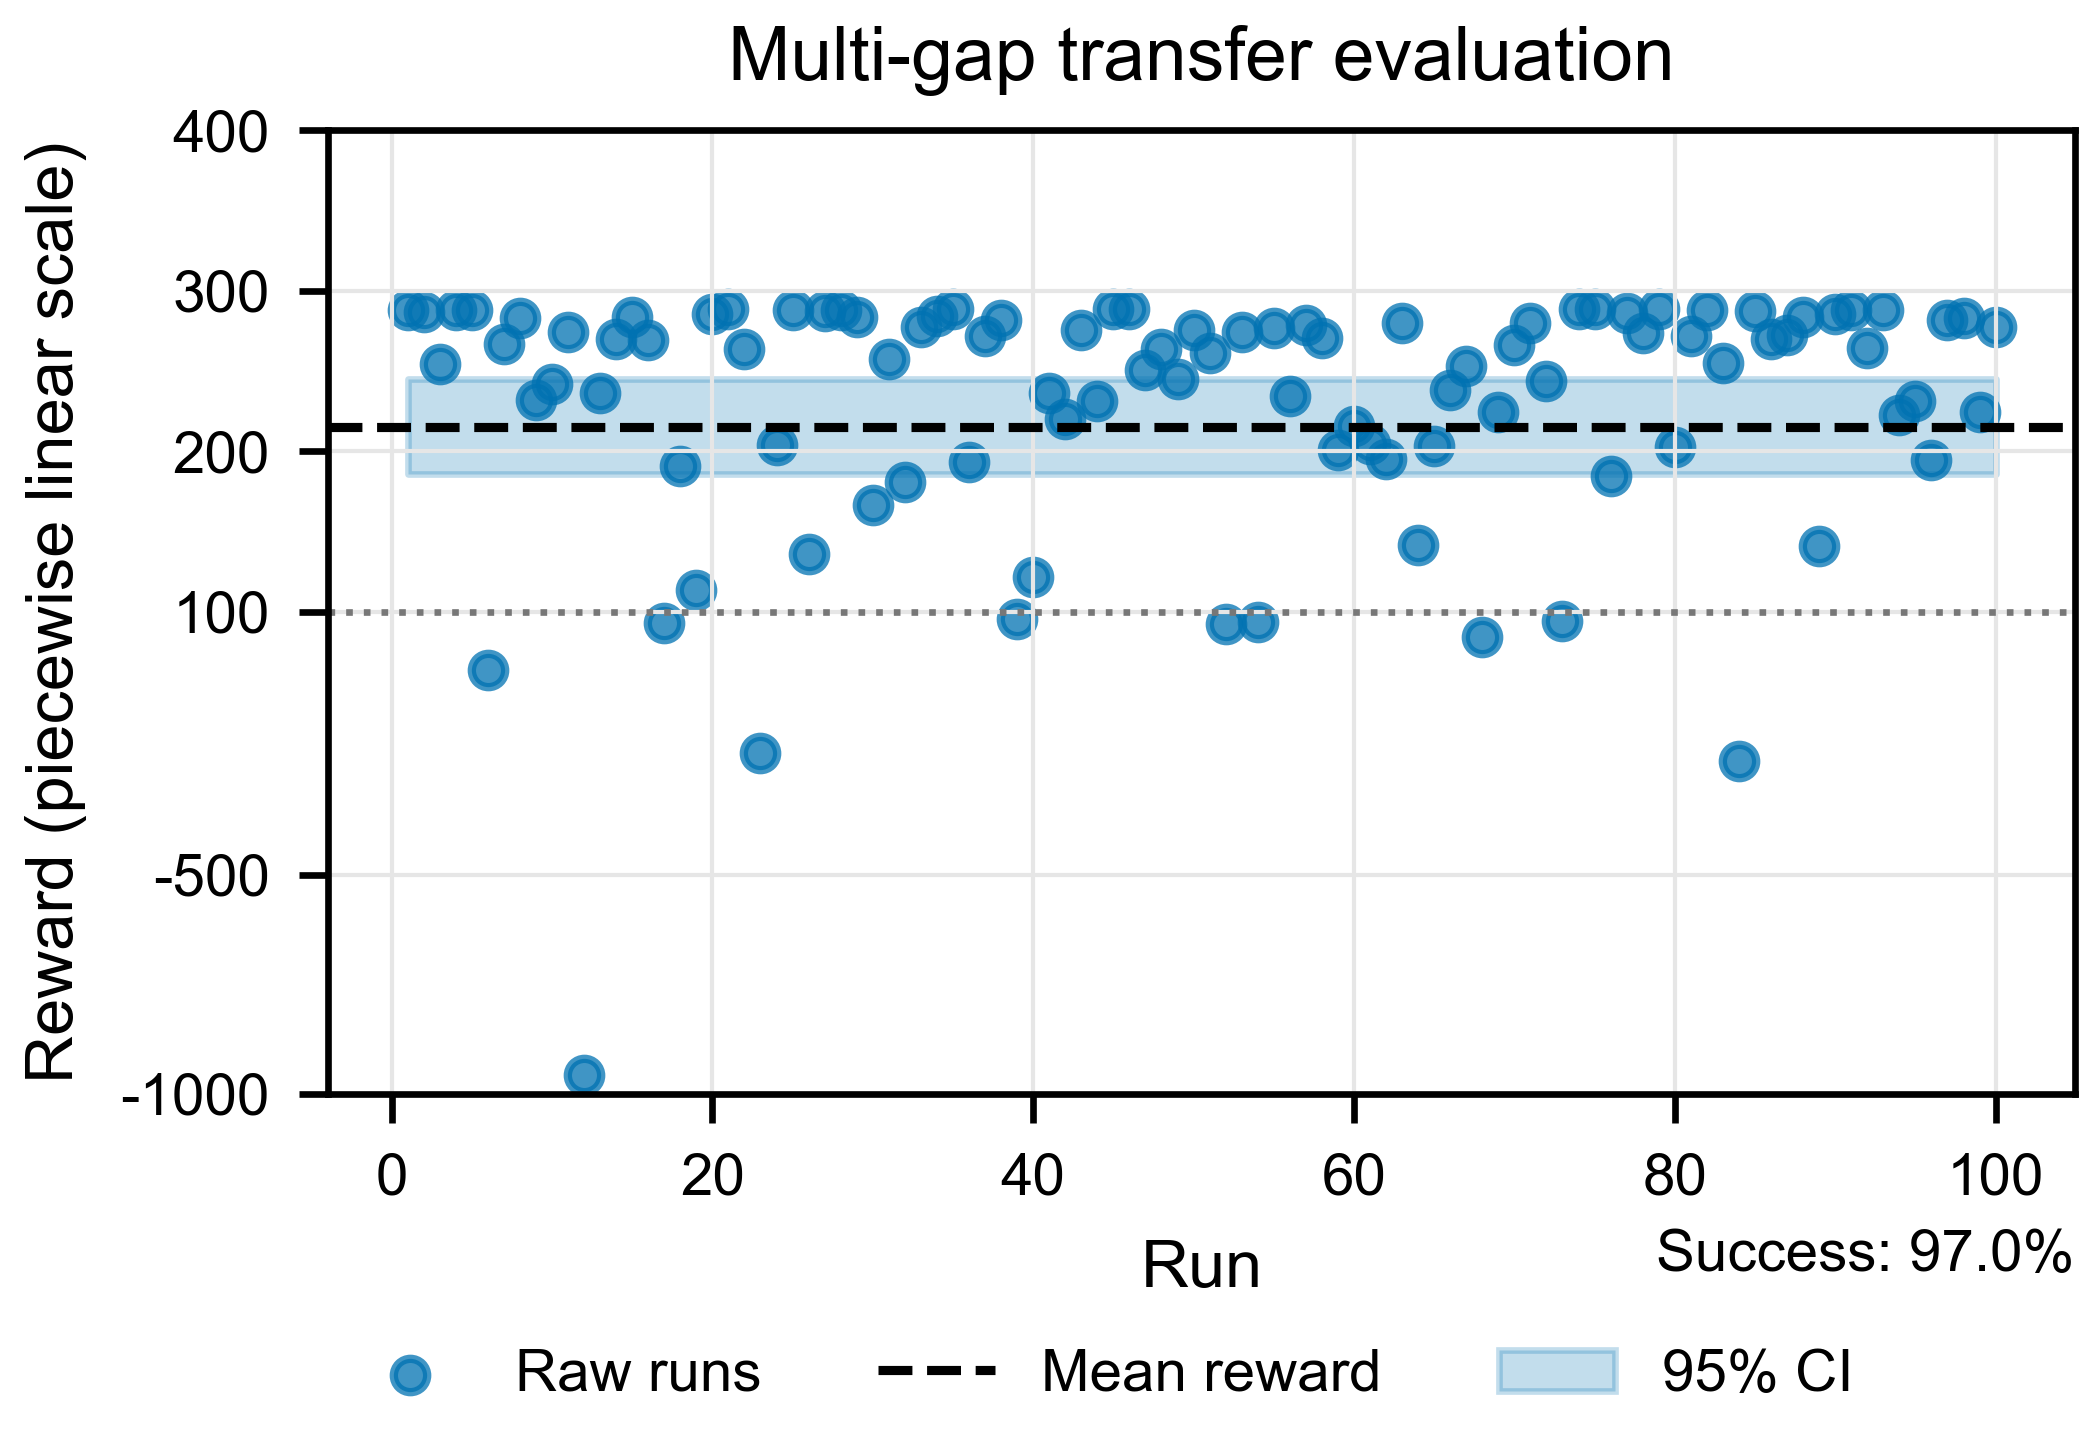
\includegraphics[width=0.92\linewidth]{fig3_multi_gap_transfer.png}
\caption{fig3\_multi\_gap\_transfer}
\label{fig:fig3-multi-gap-transfer}
\end{figure}



Fig. 6: The results of the multiple gap generalization experiments





The low-level SAC strategy was trained in a single-gap environment and then directly deployed to a dynamic multi-gap scenario. The experimental results show that it has good generalization ability in terms of safety and task completion: the success rate remains at a high level (\(\approx\)0.97). Even if the high-level selector switches, in the vast majority of cases, the low-level strategy never violates the safety boundary. These data confirm that SAC strategy generalizes beyond the training environment.



Although the reward remained consistent with that in the single-gap experiment in most cases, in some difficult cases, the strategy might deteriorate and lead to failure. Analysis of the experimental data of failures and low rewards, the failures mainly arise from two factors: the repeated decision-making caused by the complex environment, resulting in a long decision-making time exceeding the maximum simulation time and leading to task failure; and the decision being at a local optimal solution, resulting in overly cautious actions and excessive time spent, thereby causing a serious deduction in the step term. The reasons for the decline in generalization performance may be that too little environmental information was input during training, and only the instantaneous state was focused on while ignoring the changes on the time scale.



\section{High-level decision-making Ablation experiment}



\begin{figure}[H]
\centering
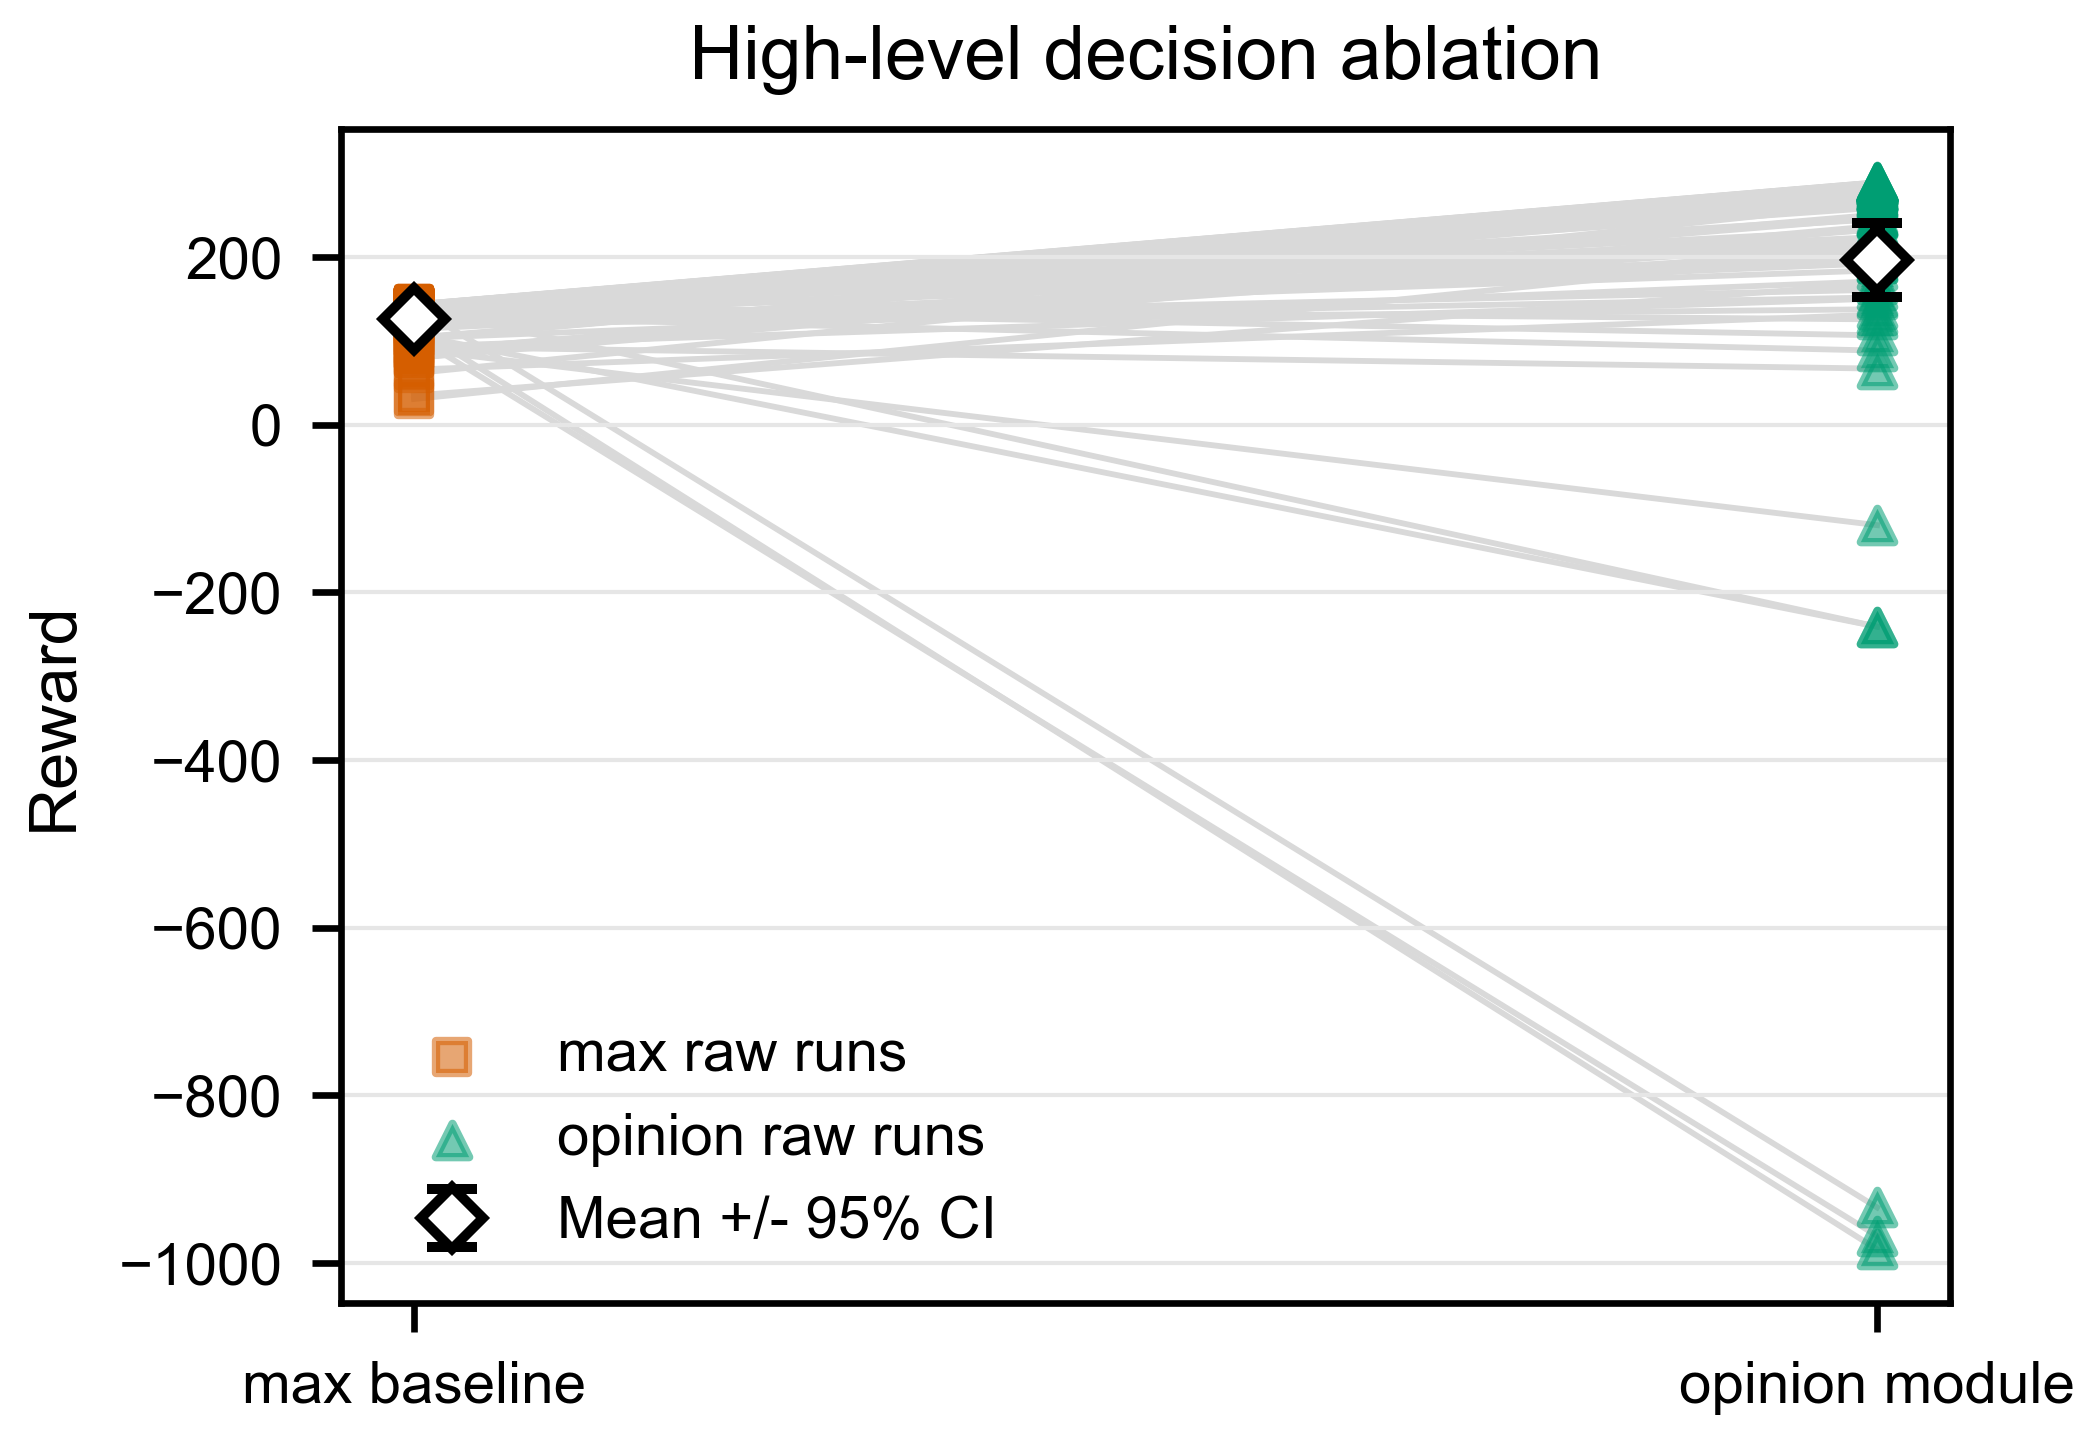
\includegraphics[width=0.92\linewidth]{fig4_multi_gap_ablation.png}
\caption{fig4\_multi\_gap\_ablation}
\label{fig:fig4-multi-gap-ablation}
\end{figure}



Fig. 7: Comparison of high-level strategy rewards between Opinion and Max





The ablation compares two high-level decision-making strategies: the opinion-dynamics strategy (which provides recommendations based on the attention mechanism) and the max-score strategy (which selects the gap that maximizes a certain indicator), the opinion-dynamics strategy achieved significantly higher average rewards (+55.3\%), indicating that the gap selected by the opinion-dynamics strategy is superior to the max-score strategy in terms of safety, stability, and overall returns. Although the max-score strategy completed tasks in a shorter time (average 8.2 seconds compared to 12.6 seconds) in some cases, its low rewards mainly resulted from larger safety penalties and less smooth control, reflecting that the selected gap might be too aggressive or not conducive to the smooth execution of the low-level strategy. In terms of the number of switches, the opinion-dynamics strategy had an fewer switches on average (0.61 vs 0.76), indicating that the gap suggestions provided by the opinion-dynamics strategy have better temporal consistency, reducing the control jitter caused by frequent switching of targets, and facilitating the improvement of passenger comfort and algorithm stability. The success rate of the opinion-dynamics strategy (97\%) was slightly lowerer than that of the max-score strategy (100\%), mainly due to timeout failures caused by exceeding the maximum simulation time. In summary, the opinion-dynamics strategy outperformed the max-score strategy in terms of total rewards and switch stability, verifying that the high-level decision-making based on attention can more effectively guide the low-level strategy and generate more stable lane-changing behaviors.



\begin{longtable}{p{0.22\linewidth}p{0.22\linewidth}p{0.22\linewidth}p{0.22\linewidth}}
\toprule
Metric & Opinion Strategy & Max Strategy & Improvement \\
\midrule
\textbf{Mean Episode Reward} (\(\bar{R}\)) & 196.8 & 126.7 & \textbf{+55.3\%} \\
\textbf{Mean Switch Count} & 0.61 & 0.76 & \textbf{-19.7\%} \\
\textbf{Mean Completion Time (s)} & 12.6 & 8.2 & — \\
\textbf{Success Rate} & \textbf{97\%} & 100\% & — \\
\bottomrule
\end{longtable}



\chapter{Conclusions}





The two-layer opinion dynamics framework provides an interpretable and experimentally verifiable method for autonomous lane merging. The upper layer makes a choice in the local candidate gap by smoothing the confidence difference and self-updating attention; the lower layer executes the selected action through objective gap bias, learned or analytic attention, opinion-driven target point interpolation, and tracking control with safety obstacle avoidance.



Comprehensive experiments show that SAC lower strategy trained in a single-gap scenario using this framework can converge stably and significantly outperform the manually designed RBF controller, verifying the advantages of learning-based strategies in balancing efficiency and safety. In the multi-gap generalization test, the lower strategy maintains a high safety success rate, demonstrating its certain generalization ability; however, in some difficult scenarios, there is reduced efficiency or timeout failures, indicating that the current lower strategy's adaptability to dynamic switching environments is still insufficient. This limitation mainly arises from the lack of temporal context information in the state space during training and the inability of the lower layer to perceive the switching of the upper layer or detect the unfeasibility of the gap. The decision-making ablation experiment of the attention-based Opinion strategy shows that it outperforms the max-score strategy in total rewards and has fewer switching times, indicating that reasonable upper-layer guidance can effectively improve overall performance.

% BEGIN GENERATED DOCX APPENDICES

\appendix

\chapter{Project Outline}

Learning Decision Dynamics for Multi-Robot Teams: Hierarchical Strategy and Control

Project Scope

This research project is fundamentally situated at the intersection of multi-agent systems, nonlinear control theory, and machine learning. The primary scope encompasses the design, mathematical formulation, software implementation, and extensive simulation-based evaluation of a novel hierarchical framework. Specifically, the project will focus on employing Reinforcement Learning (RL) techniques to dynamically optimize the governing parameters of a nonlinear control system, which dictates the strategic opinion dynamics and physical behavior of a multi-robot team. The scope includes establishing a robust simulation environment (e.g., using ROS and Python) to model complex, interactive scenarios where robots must navigate the trade-offs between cooperative consensus and competitive dissensus. The boundary of this project is strictly confined to computational modeling and algorithmic simulation; it explicitly excludes any hardware deployment, physical robot trials, real-world outdoor testing, or human-in-the-loop experiments. All datasets generated and utilized will be purely synthetic.

Motivation

The deployment of multi-robot teams in highly dynamic and unpredictable environments---such as autonomous driving, search and rescue operations, and automated logistics---presents a formidable challenge. Traditional control strategies often rely on fixed, pre-computed parameters for their nonlinear dynamics models. While these deterministic approaches work well in static scenarios, they critically lack the flexibility needed when the environment rapidly shifts, or when the team needs to fluidly transition between cooperative and competitive behaviors. Furthermore, there is often a distinct disconnect between high-level strategic decision-making (e.g., task allocation) and low-level physical control (e.g., collision avoidance). By introducing state-of-the-art Reinforcement Learning methods to continuously and adaptively optimize the parameters of the nonlinear control systems, this project aims to bridge that critical gap. The motivation is to endow the robotic team with the "intelligence" to learn optimal decision dynamics directly from experiential feedback, thereby significantly enhancing the system's overall efficiency, safety, and adaptability in complex, multi-agent interactions.

Aim

Aim: The overarching aim of this research project is to develop, integrate, and extensively validate a comprehensive, hierarchical decision-making and control framework for multi-robot systems. This framework will leverage Reinforcement Learning algorithms to intelligently tune the parameters of a nonlinear control system, enabling distributed agents to reach rapid strategic consensus or dissensus while strictly adhering to safety-critical physical constraints in a fully simulated, highly dynamic environment.

Objectives

To realize the overarching aim, this project is broken down into the following specific, measurable objectives:

Mathematical Formulation: To construct a rigorous strategic-level mathematical model utilizing nonlinear opinion dynamics that dictates distributed consensus, role assignments, and task allocation among the multi-robot team.

RL-Based Parameter Optimization: To design and train a Reinforcement Learning agent (e.g., utilizing algorithms such as Proximal Policy Optimization or Soft Actor-Critic) dedicated to dynamically optimizing the critical tuning parameters of the nonlinear control system, allowing the team's cooperative/competitive behavior to adapt in real-time to environmental stimuli.

Safe Control Execution: To develop an execution-level control strategy (incorporating methods like Control Barrier Functions) that securely translates high-level strategic objectives into collision-free kinodynamic trajectories, ensuring that physical constraints are never violated.

System Integration: To seamlessly integrate the high-level RL-driven decision dynamics with the low-level safety controllers within a robust, multi-agent simulation framework (e.g., using ROS 2 and Python-based physics engines).

Performance Evaluation: To conduct exhaustive simulation trials across varied operational scenarios, benchmarking the RL-optimized system against traditional fixed-parameter baseline controllers by evaluating metrics such as convergence speed, safety violation rates, and overall task efficiency.

\chapter{Risk Assessment}

General Risk Assessment Form

\begin{small}
\begin{longtable}{p{0.15\linewidth}p{0.15\linewidth}p{0.15\linewidth}p{0.15\linewidth}p{0.15\linewidth}p{0.15\linewidth}}
\toprule
Date: (1) 2026.7.1 & Assessed by: (2) Junyi Lei & Checked / Validated* by: (3) & Location:  (4) Home & Assessment ref no (5) & Review date: (6) \\
\midrule
Task / premises: (7) Software development, algorithm simulation (RL for nonlinear control), data analysis, and report writing. &  &  &  &  &  \\
\bottomrule
\end{longtable}
\end{small}

\begin{small}
\begin{longtable}{p{0.15\linewidth}p{0.15\linewidth}p{0.15\linewidth}p{0.15\linewidth}p{0.15\linewidth}p{0.15\linewidth}}
\toprule
Activity (8) & Hazard (9) & Who might be harmed and how (10) & Existing measures to control risk (11) & Risk rating (12) & Result (13) \\
\midrule
Working from home & Lone working & Home working staff Isolated, & Please refer to the University Lone Working policy and guidance for more information Please refer to the new University Working at Home guidance Please refer to the new University Wellbeing Support website Staff are able to have regular direct contact with line manager and colleagues via phone, Teams, Zoom or email & Low & A \\
Working from home & Poor posture, repetitive movements, eye strain, from long periods looking at DSE (display screen equipment) & Staff, students, visitors Back strain (due to poor posture). Repetitive Strain Injury (RSI) to upper limbs. Eye strain. & Please refer to the DSE policy, guidance and poster for more information on how to set up your workstation properly Complete DSE Self-Assessment for your home working at least every 2 years but sooner if any changes or pain is experienced. Complete Homeworking self-assessment checklist Set up workstation to a comfortable position with good lighting and natural light where possible Take regular breaks away from the screen Regularly stretch your arms, back, neck, wrists and hands to avoid repetitive strain injuries. Refer to seated exercises Set up a desktop working space where possible and try to avoid working on a laptop without a docking station, separate keyboard or mouse Small equipment purchases of up to £50 to assist with working from home, contact local administration for more details. If experiencing ill-health issues contact your local DSE assessor or local safety advisor who will perform a full DSE assessment. Occupational health referral where issues cannot be resolved from full DSE assessment. DSE users should have regular eye tests, follow guidance FSE run monthly DSE awareness sessions on Teams & Low & A \\
Working from home & Stress / Wellbeing & Home working staff Psychosocial effects Work / Life imbalance Anxiety Poor performance Fatigue \& Tiredness & Please refer to Stress Prevention and Management toolkit for policies and guidance Please refer to new University guidance for Managing teams working from home Please refer to Seven rules of home working published by AMBS Please refer to Guidance for Managers and Guidance for Staff Complete training Work Related Stress: Identification, Prevention \& Management (Online) The University Stress Assessment tool can be used to highlight the main factors for an individual that are recognised as having the potential to lead to work-related stress Projects, work plans and objectives to be discussed and agreed with line manager regularly Refer to full FSE Stress Risk Assessment Regular contact meetings with manager and peers via Teams, Zoom, email and phone Define working hours, set a start \& close daily routine, and prioritise your tasks. Individual may self-refer to Occupational Health Service or to the Counselling and Mental Health Service Manager / Employee consultation, wellbeing focused & Low & A \\
Use of electrical appliances & Misuse of electrical appliance, faulted electrical appliance. & Home working staff Electric shock, burns and fire & All office equipment used in accordance with the manufacturer’s instructions Visual checks before use to make sure equipment, cables and free from defects University IT equipment brought home should already be PAT tested, small electrical items can be tested through the FSE I\&F team The domestic electrical supply and equipment owned by the employee is the responsibility of the employee to maintain Liquid spills cleaned up immediately Defective plugs, cables and equipment should be taken out of use & Med & A \\
Moving around the home office & Obstructions and trip hazards & Home working staff Slips, trips and falls causing physical injury & Floors and walkways kept clear of items, e.g. boxes, packaging, equipment etc Furniture is arranged such that movement of people and equipment are not restricted Make sure all areas have good level of lighting Reasonable standards of housekeeping maintained Trailing cables positioned neatly away from walkways Cabinet drawers and doors kept closed when not in use & Med & A \\
Working from home & Fire & Staff Home Working Risk of burns, smoke inhalation, asphyxiation & In the event of a fire evacuate out of the building and call the fire brigade on 999 All waste, including combustible waste, removed regularly Heaters located away from combustible materials and switched off when not in use, don’t leave heaters unattended Avoid daisy chaining and do not overload extension leads Test smoke alarm routinely and replace batteries every 6-12 months Please refer to fire brigade Home Fire Safety and Smoke Alarms & Med & A \\
\bottomrule
\end{longtable}
\end{small}

\begin{small}
\begin{longtable}{p{0.18\linewidth}p{0.18\linewidth}p{0.18\linewidth}p{0.18\linewidth}p{0.18\linewidth}}
\toprule
Action plan (14) &  &  &  &  \\
\midrule
Ref No & Further action required & Action by whom & Action by when & Done \\
1 & DSE Self-Assessment: Complete the workstation self-assessment to prevent physical strain (neck/back/eyes) during extended ROS 2 programming and RL training sessions. & Student & Week1 &  \\
2 & Workload \& Stress Management: Implement regular timeline reviews with the supervisor to manage stress, ensuring the project milestones and dissertation writing remain on track for the final September submission deadline. & Student & Week2-3 &  \\
3 & Data Backup: Establish automated version control and secure backups for simulation logs, RL models, and draft reports to prevent data loss due to computer failure. & Student & Week1 &  \\
4 & Equipment Safety Check: Visually inspect laptop, chargers, and extension leads before intensive simulation sessions to mitigate overheating and fire risks. & Student & Week1 &  \\
\bottomrule
\end{longtable}
\end{small}

\begin{small}
\begin{longtable}{p{0.28\linewidth}p{0.28\linewidth}}
\toprule
I have read and I understand the content of this office risk assessment and I will comply with this Risk Assessment &  \\
\midrule
Name (print) & Signature \\
\bottomrule
\end{longtable}
\end{small}

\chapter{Experimental Parameter Summary}

\begin{small}
\begin{longtable}{p{0.23\linewidth}p{0.23\linewidth}p{0.23\linewidth}p{0.23\linewidth}}
\toprule
Category & Symbol & Value & Description \\
\midrule
Simulation & \(T\) & \(40.0\,\mathrm{s}\) & Episode duration \\
Simulation & \(\Delta t\) & \(0.05\,\mathrm{s}\) & Integration interval \\
Road & \(W\) & \(4.0\,\mathrm{m}\) & Lane width \\
Road & \(y_O,y_T\) & \(2.0\,\mathrm{m},6.0\,\mathrm{m}\) & Original and target lane centers \\
Vehicle & \(L\) & \(2.8\,\mathrm{m}\) & Vehicle wheelbase \\
Safety & \(r\) & \(1.5\,\mathrm{m}\) & Collision boundary radius \\
Single-gap initial state & \(x_F(0),x_R(0)\) & \(30.0\,\mathrm{m},15.0\,\mathrm{m}\) & Front and rear target-vehicle initial positions \\
Single-gap initial state & \(x_e(0)\) & \(20.0+\mathcal{U}(-5.0,5.0)\,\mathrm{m}\) & Ego randomized initial position \\
Single-gap rear motion & \(t_y\) & \(20.0\,\mathrm{s}\) & Yielding starts after this time \\
Single-gap rear motion & \(A_s,P_s\) & \(4.0\,\mathrm{m / s},6.0\,\mathrm{s}\) & Sinusoidal velocity amplitude and period before yielding \\
Single-gap rear motion & \(g_{\mathrm{yield}}\) & \(20.0\,\mathrm{m}\) & Desired front-rear gap after yielding \\
Single-gap rear motion & \(a_R\) clip & \([-5.0,2.0]\,\mathrm{m / s^2}\) & Rear-vehicle acceleration bounds after yielding \\
Single-gap low level & \(g_{\mathrm{safe}}\) & \(10.0\,\mathrm{m}\) & Safe-gap threshold for single-gap training \\
SAC training & \(N_{\mathrm{ep}}\) & \(200\) & Training episodes \\
SAC training & \(N_{\mathrm{rand}}\) & \(1000\) steps & Initial random exploration steps \\
SAC training & \(\gamma,\tau\) & \(0.99,0.005\) & Discount factor and target-network update rate \\
SAC training & \(B_{\mathrm{batch}}\) & \(256\) & Batch size \\
SAC training & \(\mathcal{D}\) & \(200000\) & Replay-buffer capacity \\
SAC training & \(\eta_{\pi},\eta_Q,\eta_{\alpha}\) & \(3\times10^{-4}\) & Policy, Q-network, and entropy-temperature learning rates \\
SAC training & \(H\) & \(256\) & Hidden-layer width \\
SAC action & \(u_{\min},u_{\max}\) & \(0.0,3.0\) & Learned attention range \\
Single-gap evaluation & \(N_{\mathrm{eval}}\) & \(10\) & Repeated value-comparison runs \\
RBF baseline & \(u_{\mathrm{base}},u_{\mathrm{amp}}\) & \(0.2,2.5\) & Hand-designed attention baseline parameters \\
RBF baseline & \(\sigma_d,\sigma_v\) & \(2.0,1.5\) & Single-gap RBF position and velocity bandwidths \\
Multi-gap fleet & \(N\) & \(5\) & Number of target-lane vehicles \\
Multi-gap fleet & \(N_g\) & \(4\) & Number of physical gaps \\
Multi-gap initial state & \(x_i(0)\) & \(48.0-(i-1)8.0\,\mathrm{m}\) & Target-vehicle initial positions \\
Multi-gap initial state & \(x_e(0)\) & \(30.0+\mathcal{U}(-10.0,10.0)\,\mathrm{m}\) & Ego randomized initial position \\
Multi-gap schedule & \(g_0\) & \(8.0\,\mathrm{m}\) & Base desired gap \\
Multi-gap schedule & \(T_g\) & \(4.0\,\mathrm{s}\) & Gap adjustment interval \\
Multi-gap schedule & \(\mathcal{M}\) & \(\{0.75,1.0,1.25,1.5\}\) & Desired-gap multiplier set \\
Multi-gap schedule & \(N_{\mathrm{chg}}\) & \(\leq2\) gaps / period & Maximum changed gaps per period \\
Multi-gap following & \(k_p^g,k_d^g\) & \(0.55,1.05\) & Gap-tracking gains \\
Multi-gap following & \(a_{\max}^g\) & \(4.0\,\mathrm{m / s^2}\) & Target-vehicle acceleration limit \\
High-level opinion & \(d_y,\alpha_y\) & \(2.5,10.0\) & High-level damping and sensitivity \\
High-level attention & \(\tau_h,U_{\max},K_h,n\) & \(1.0,1.5,0.2,2.0\) & Self-updating attention parameters \\
High-level decision & \(\theta_y\) & \(0.18\) & Waiting-band decision threshold \\
Multi-gap confidence & \(\sigma_d,\sigma_v\) & \(4.0,2.5\) & Confidence bandwidths for local gap comparison \\
Low-level opinion & \(g_{\mathrm{safe}},k_g,k_v\) & \(5.0\,\mathrm{m},0.2,0.1\) & Gap-bias parameters in multi-gap execution \\
Low-level opinion & \(d_z,\alpha_z\) & \(2.0,2.0\) & Low-level opinion damping and sensitivity \\
Multi-gap evaluation & \(N_{\mathrm{test}}\) & \(100\) & Random repeated test runs \\
Physical input & \(a\) clip & \([-5.0,5.0]\,\mathrm{m / s^2}\) & Ego acceleration bounds \\
Physical input & \(\omega\) clip & \([-0.8,0.8]\,\mathrm{rad / s}\) & Ego steering-rate bounds \\
\bottomrule
\end{longtable}
\end{small}

% END GENERATED DOCX APPENDICES

\printbibliography

\end{document}
